\section{Determinant (\S3.1)}
Getal (scalar) dat hoort bij een $(n \times n)$ matrix.

\subsection{Definitie}
\begin{enumerate}
	\item[In 2D] det $\begin{pmatrix} a & b \\ c & d \end{pmatrix} \to a \cdot d - c \cdot b$

	\item[In 3D] Gaat via het ontwikkelen van de matrix. \index{Ontwikkelen matrix} Een element in de matrix vermenigvuldigen met de determinant van de sub-matrix die er tegenover staat. Dit is de sub-matrix die wordt gevormd door alle elementen zonder de elementen in dezelfde rij en kolom van het element.
	\[\mbox{det} \begin{pmatrix}
		a_{11} & a_{12} & a_{13} \\
		a_{21} & a_{22} & a_{23} \\
		a_{31} & a_{32} & a_{33}
	\end{pmatrix} \to a_{11} \cdot \mbox{det} \begin{pmatrix} a_{22} & a_{23} \\ a_{32} & a_{33} \end{pmatrix} - a_{12} \cdot \mbox{det} \begin{pmatrix} a_{21} & a_{23} \\ a_{31} & a_{33} \end{pmatrix} + a_{13} \cdot \mbox{det} \begin{pmatrix} a_{21} & a_{22} \\ a_{31} & a_{32} \end{pmatrix}\]
	De ontwikkeling ziet er dus zo uit:
	\[ \begin{pmatrix}
		\mathbf{a_{11}} && \\
		& a_{22} & a_{23} \\
		& a_{32} & a_{33}
	\end{pmatrix}, \begin{pmatrix}
		& \mathbf{a_{12}} & \\
		a_{21} && a_{23} \\
		a_{31} && a_{33}
	\end{pmatrix}, \begin{pmatrix}
		&& \mathbf{a_{13}} \\
		a_{21} & a_{22} & \\
		a_{31} & a_{32} &
	\end{pmatrix}\]
	Om te bepalen of een term positief of negatief is gebruik je de volgende matrix, bij grotere matrices breidt je hem uit volgens hetzelfde patroon:
	\[ \begin{pmatrix}
		+ & - & + \\
		- & + & - \\
		+ & - & +
	\end{pmatrix}\]
	
	\paragraph{Voorbeeld} Ontwikkelen langs eerste rij
	\begin{eqnarray*}
		\mbox{det} \begin{pmatrix*}[r] 1 & -2 & 0 \\ 2 & 1 & 4 \\ 0 & 1 & 2 \end{pmatrix*} &=& 1 \cdot \mbox{det} \begin{pmatrix} 1 & 4 \\ 1 & 2 \end{pmatrix} - (-2) \cdot \mbox{det} \begin{pmatrix} 2 & 4 \\ 0 & 2 \end{pmatrix} + 0 \cdot \begin{pmatrix} 2 & 1 \\ 0 & 1 \end{pmatrix} \\
		&=& 1 \cdot (1 \cdot 2 - 1 \cdot 4) + 2 \cdot (2 \cdot 2 - 0 \cdot 4) + 0 \\
		&=& -2 + 2 \cdot 4 \\
		&=& 6
	\end{eqnarray*}
	\paragraph{Voorbeeld} Ontwikkelen langs eerste kolom
	\begin{eqnarray*}
		&=& 1 \cdot \mbox{det} \begin{pmatrix} 1 & 4 \\ 1 & 2 \end{pmatrix} - 2 \cdot \mbox{det} \begin{pmatrix*}[r] -2 & 0 \\ 1 & 2 \end{pmatrix*} + 0 \cdot \mbox{det} \begin{pmatrix*} -2 & 0 \\ 1 & 4 \end{pmatrix*} \\
		&=& 1 \cdot (-2) - 2 \cdot (-4 - 0) + 0 \\
		&=& -2 + 8 = 6
	\end{eqnarray*}

	\item[In 4D] Je kiest een rij of kolom uit de matrix om langs te ontwikkelen, het is het handigste om te kiezen voor de rij of kolom met de meeste nullen er in omdat dit het minste werk oplevert. De rij of kolom waar langs wordt ontwikkeld wordt aangegeven met een lijn vanaf nu.
	\[ \mbox{det} \begin{pmatrix*}[r]
		1 & -2 & 0 & 1 \\
		0 & 2 & 1 & -3 \\
		1 & 0 & 0 & -2 \\
		0 & 1 & -4 & -2
	\end{pmatrix*}\]
	Deze matrix kun je ontwikkelen langs de 3e rij:
	\begin{eqnarray*}
		&&1 \cdot \mbox{det} \left(\!\begin{array}{rrr}
			-2 & 0 & 1 \\ \hline
			2 & 1 & -3 \\
			1 & -4 & 2
		\end{array}\!\right) - 0 \cdot \mbox{det} + 0 \cdot \mbox{det} - (-2) \cdot \mbox{det} \left(\!\begin{array}{r|rr}
			1 & -2 & 0 \\
			0 & 2 & 1 \\
			0 & 1 & -4
		\end{array}\!\right) \\
		&=& -2 \cdot \mbox{det} \begin{pmatrix*}[r] 1 & -3 \\ -4 & 2 \end{pmatrix*} - 0 + 1 \cdot \mbox{det} \begin{pmatrix*}[r] 2 & 1 \\ 1 & -4 \end{pmatrix*} + 1 \cdot \mbox{det} \begin{pmatrix*}[r] 2 & 1 \\ 1 & -4 \end{pmatrix*} + 0 + 0 \\
		&=& -2 \cdot (1 \cdot 2 - (-4) \cdot (-3)) + 1 \cdot (2 \cdot -4 - 1 \cdot 1) + 1 \cdot (2 \cdot -4 - 1 \cdot 1) \\
		&=& -2 \cdot -10 + 1 \cdot -9 + 1 \cdot -9 = 20 - 9 - 9 = 2
	\end{eqnarray*}
\end{enumerate}

\subsection{Speciale gevallen}
\begin{enumerate}
	\item Diagonaal matrix. De determinant is het product van de elementen op de hoofddiagonaal.
	\[ A = \begin{pmatrix}
		3 && \sigma \\
		& -2 & \\
		\sigma && 1
	\end{pmatrix} \to \mbox{det}(A) = 3 \cdot (-2) \cdot 1 = -6 \]
	
	\item Driehoeks matrix. Hierbij is de determinant ook het product van de element op de hoofddiagonaal.
	\[A = \begin{pmatrix*}[r]
		3 & 0 & 0 \\
		2 & -2 & 0 \\
		1 & -4 & 1
	\end{pmatrix*} \to \mbox{det}(A) = 3 \cdot (-2) \cdot 1 = -6 \]
	
	\item Diagonaal blok matrix: \[\mbox{det} \begin{pmatrix}
		A_{11} & \sigma \\
		\sigma & A_{22}
	\end{pmatrix} = \mbox{det}(A_{11}) \cdot \mbox{det}(A_{22}) \]
	Als de sub-matrix slechts een enkel getal is dan is dat getal de determinant.
	
	\paragraph{Voorbeeld}
	\[
		\mbox{det} \left(\!\begin{array}{rr|rr}
			1 & -1 & 0 & 0 \\
			2 & 0 & 0 & 0 \\ \hline
			0 & 0 & 1 & 4 \\
			0 & 0 & -6 & 0
		\end{array}\!\right)
		= \mbox{det}\begin{pmatrix*} 1 & -1 \\ 2 & 0 \end{pmatrix*} \cdot \mbox{det} \begin{pmatrix*} 1 & 4 \\ -6 & 0 \end{pmatrix*}
		= 2 \cdot 24 = 48 \]
\end{enumerate}

\section{Eigenschappen van de determinant (\S3.2)}
\subsection{Toepassing 1: Stelsel onderzoek}

\paragraph{Stelling 4:} \index{Stellingen!Hoofdstuk 3!Stelling 4} Als $A^{-1}$ bestaat $\iff$ det$(A) \neq 0 \iff A \vec{x} = \vec{b}$ heeft precies \'e\'en oplossing.

Daarnaast is $A$ lineair afhankelijk als det$(A) = 0$.

\paragraph{Voorbeeld}
Heeft het volgende stelsel een oplossing?
\[ \left\{ \begin{array}{r}
	x + 2y = 1 \\
	-x + y = 2
\end{array}\right. \]
\[ A = \begin{pmatrix*}1 & 2 \\ -1 & 1 \end{pmatrix*}, \mbox{det}(A) = 1 \cdot 1 - (-1) \cdot 2 = 3 \neq 0 \]
Er is dus precies \'e\'en oplossing: via vegen geeft dit $\vec{x} = \begin{vect} -1 \\ 1 \end{vect}$. Via de inverse geeft dit $\vec{x} = A^{-1} \vec{b} = \begin{vect} -1 \\ 1 \end{vect}$.

\paragraph{Voorbeeld} Voor welke $\alpha$ is er bij het stelsel 
$\left\{ \begin{array}{r}
	x + 2y = 1 \\
	\alpha x + y = 2
\end{array}\right.$ precies \'e\'en oplossing?
\[ \mbox{det}\begin{pmatrix*}[r] 1 & 2 \\ \alpha & -2 \end{pmatrix*} = 1 \cdot -2 - \alpha -2 = -2 - 2 \alpha \neq 0\]
\[ \to 2 \alpha \neq -2 \]
\[ \alpha \neq -1 \]

\paragraph{Voorbeeld} Andere oplossing voor het probleem met constanten op pagina  \pageref{par:constantenprobleem}. Voor welke $\alpha$ is er \'e\'en oplossing? Eerst loste je dit op door schoon te vegen, nu met det$(A) \neq 0$.
\[ \left\{\begin{array}{l}
	x + y - z = 1 \\
	2x + 3y + \alpha z = 3 \\
	x + \alpha y + 3z = 2
\end{array}\right. \]
\begin{eqnarray*}
	\mbox{det} \left(\!\begin{array}{r|rr}
		1 & 1 & -1 \\
		2 & 3 & \alpha \\
		1 & \alpha & 3
	\end{array}\!\right) &=& 1 \cdot \mbox{det} \begin{pmatrix} 3 & \alpha \\ \alpha & 3 \end{pmatrix} - 2 \cdot \mbox{det} \begin{pmatrix*} 1 & -1 \\ \alpha & 3 \end{pmatrix*} + 1 \cdot \mbox{det} \begin{pmatrix*}[r] 1 & -1 \\ 3 & \alpha \end{pmatrix*} \\
	&=& 1 \cdot (9 - \alpha^2) - 2 \cdot (3 + \alpha) + 1 \cdot (\alpha +3) \\
	&=& -\alpha^2 - \alpha + 6 \neq 0
\end{eqnarray*}
Dit geeft via de ABC-formule de oplossing: $\alpha \neq -3 \wedge \alpha \neq 2$.

\subsection{Rekenregels}
\paragraph{Stelling 3:} \index{Stellingen!Hoofdstuk 3!Stelling 3}
\begin{enumerate}
	\item Rijen optellen $\to$ determinant blijft hetzelfde
	\item Rijen verwisselen $\to$ determinant $\cdot -1$. Twee keer verwisselen wordt dus weer de normale determinant.
	\item Rij $\cdot k \to$ det $\cdot k$.
	\item Rij $i = k \cdot$ Rij $j \to$ det$(A) = 0$. Dus als de rijen afhankelijk zijn dan is de determinant 0.
\end{enumerate}
Wat voor rijen geldt is ook van toepassing op kolommen.

\paragraph{Voorbeeld}
\begin{enumerate}
	\item \[ A = \begin{pmatrix} 1 & 2 \\ 3 & 4 \end{pmatrix} \to \mbox{det}(A) = 4-6 = -2 \]
	\[ \mbox{det}\begin{pmatrix} 1 & 2 & 4 & 6 \end{pmatrix} \to \mbox{det} = 6 - 8 = -2 \]
	
	\item \[ \mbox{det} \begin{pmatrix}3 & 4 \\ 1 & 2 \end{pmatrix} = 6 - 4 = 2 \]
	
	\[ \mbox{det} \begin{pmatrix*}[r]
		1 & -1 & 2 \\
		0 & 0 & 3 \\
		0 & 1 & -1
	\end{pmatrix*} \sim -\mbox{det} \begin{pmatrix*}[r]
		1 & -1 & 2 \\
		0 & 1 & -1 \\
		0 & 0 & 3
	\end{pmatrix*} = -(1 \cdot 1 \cdot 3) = -3 \]
\end{enumerate}

\paragraph{Stelling 5:} \index{Stellingen!Hoofdstuk 3!Stelling 5}
det$(A)$ = det $(A^T)$.
\paragraph{Voorbeeld}
\begin{eqnarray*}
	\mbox{det}\begin{pmatrix} 1 & 2 \\ 3 & 4 \end{pmatrix} &=& \mbox{det} \begin{pmatrix} 1 & 3 \\ 2 & 4 \end{pmatrix} \\
	1 \cdot 4 - 3 \cdot 2 = -6 &=& 1 \cdot - 2 \cdot 3 = -6
\end{eqnarray*}

\paragraph{Stelling 6:} \index{Stellingen!Hoofdstuk 3!Stelling 6}
det$(AB) =$ det$(A) \cdot$ det$(B)$ \\
det$(A + B) \neq$ det$(A)$ + det$(B)$

\paragraph{Voorbeeld}
\[ A = \begin{pmatrix} 6 & 1 \\ 3 & 2 \end{pmatrix}, B = \begin{pmatrix} 4 & 3 \\ 1 & 2 \end{pmatrix}, AB = \begin{pmatrix} 25 & 20 \\ 14 & 13 \end{pmatrix} \]
\[ \mbox{det}(A) = 12 - 3 = 9 \]
\[ \mbox{det}(B) = 8 - 3 = 5 \]
\[ \mbox{det}(AB) = 45 = 9 \cdot 5 \]

\paragraph{Voorbeeld}\[ A + B = \begin{pmatrix} 10 & 4 \\ 4 & 4 \end{pmatrix} \]
\[ \mbox{det}(A+B) = 40-16 = 24 \neq 9 + 5\]

\section{Cramer's regel (\S3.3)}
\subsection{Toepassing 2: losse componenten $\vec{x}$ berekenen}
Los op $A \vec{x} = \vec{b} \to x_i = \frac{\mbox{det}A_i(\vec{b})}{\mbox{det}A}$
\[A_i(\vec{b}): \begin{pmatrix}
	\vdots & \vdots & & \vdots & \vdots & & \vdots \\
	\vec{a_1} & \vec{a_2} & \cdots & \vec{b} & \vec{a_{i + 1}} & \cdots & \vec{a_n} \\
	\vdots & \vdots & & \vdots & \vdots & & \vdots
\end{pmatrix}\]
Dit houdt dus in dat de $i^e$ kolom van $A$ wordt vervangen door $\vec{b}$.

\paragraph{Voorbeeld}
\[ \left\{\begin{array}{l}
	3x - 2y = 6 \\
	-5x + 4y = 8
\end{array}\right. \to A = \begin{pmatrix*}[r] 3 & -2 \\ -5 & 4 \end{pmatrix*}, \vec{b} = \begin{vect} 6 \\ 8 \end{vect} \]
\[ \mbox{det}(A) = 3 \cdot 4 - (-5) \cdot (-2) = 12 - 10 = 2 \]
\begin{eqnarray*}
	A_1(\vec{b}) = \begin{pmatrix} \mathbf{6} & -2 \\ \mathbf{8} & 4 \end{pmatrix} &\to& \mbox{det}(A_1(\vec{b})) = 6 \cdot 4 - 8 \cdot (-2) = 24 + 16 = 40 \\
	&\to& x_1 = \frac{40}{2} = 20 \\
	A_2(\vec{b}) = \begin{pmatrix*}[r] 3 & \mathbf{6} \\ -5 & \mathbf{8}\end{pmatrix*} &\to& \mbox{det}(A_1(\vec{b})) = 3 \cdot 8 - (-5) \cdot 6 = 24 + 30 = 54 \\
		&\to& x_2 = \frac{54}{2} = 27
\end{eqnarray*}
\[ \vec{x} = \begin{vect} 20 \\ 27 \end{vect} \]

\paragraph{Voorbeeld} Wanneer is dit daadwerkelijk handig? Als je maar een element uit de vector van variabelen hoeft te hebben. Wat is bij de volgende vergelijking de waarde van $x_1$?
\[ \left(\!\begin{array}{rrr}
	3 & -2 & 1 \\
	3 & 1 & 5 \\
	2 & -5 & 0 \\ \hline
\end{array}\!\right) \vec{x} = \begin{vect} 7 \\ 2 \\ -1  \end{vect} \]
\[ \mbox{det}(A) = 2 \cdot \mbox{det}\begin{pmatrix*}[r] -2 & 1 \\ 1 & 5 \end{pmatrix*} - (-5) \cdot \mbox{det}\begin{pmatrix} 5 & 1 \\ 3 & 5 \end{pmatrix} + 0 = 88 \]
\[ \mbox{det}(A_1(\vec{b})) = \mbox{det} \left(\!\begin{array}{rrr|}
	\mathbf{7} & -2 & 1 \\
	\mathbf{2} & 1 & 5 \\
	\mathbf{-1} & -5 & 0 
\end{array}\,\right) = 1 \cdot \mbox{det}\begin{pmatrix*}[r] 2 & 1 \\ -1 & -5 \end{pmatrix*} - 5 \cdot \mbox{det}\begin{pmatrix*} 7 & -2 \\ -1 & -5 \end{pmatrix*} + 0 = 176 \]
\[ \to x_1 = \frac{176}{88} = 2 \]

\subsection{Toepassing 3: lineaire afbeeldingen}
$T: \vec{x} \to A \vec{x}$ hierbij kan je origineel een gebied $\mathcal{S}$ zijn. Bij $T(\mathcal{S})$ heeft dit de volgende eigenschappen:
\begin{enumerate}
	\item[2D] opp $T(\mathcal{S}) = | \mbox{det}(A)| \cdot \mbox{opp } \mathcal{S}$
	\item[3D] vol $T(\mathcal{S}) = | \mbox{det}(A)| \cdot \mbox{vol } \mathcal{S}$
\end{enumerate}

\paragraph{Voorbeeld} Dit voorbeeld is afgebeeld in \autoref{fig:linafb}.
\[ A = \begin{pmatrix} 1 & 3 \\ 2 & 1 \end{pmatrix}, \mathcal{S} = \begin{pmatrix} 0 & 0 & 1 & 1 \\ 0 & 1 & 0 & 1 \end{pmatrix}, \mbox{opp }\mathcal{S} = 1 \]
\[ A \begin{vect} 1 \\ 0 \end{vect} = \begin{pmatrix} 1 & 3 \\ 2 & 1 \end{pmatrix} \begin{vect} 1 \\ 0 \end{vect} = \begin{vect} 1 \\ 2 \end{vect} \]
\[ A \begin{vect} 0 \\ 1 \end{vect} = \begin{pmatrix} 1 & 3 \\ 2 & 1 \end{pmatrix} \begin{vect} 0 \\ 1 \end{vect} = \begin{vect} 3 \\ 1 \end{vect} \]
\[ A \begin{vect} 1 \\ 1 \end{vect} = \begin{pmatrix} 1 & 3 \\ 2 & 1 \end{pmatrix} \begin{vect} 1 \\ 1 \end{vect} = \begin{vect} 4 \\ 3 \end{vect} \]
\[ \mbox{opp } T(\mathcal{S}) = |\mbox{det}(A)| \cdot \mbox{opp } \mathcal{S} = |-5| \cdot 1 = 5 \]

\begin{figure}[h!]
	\centering
	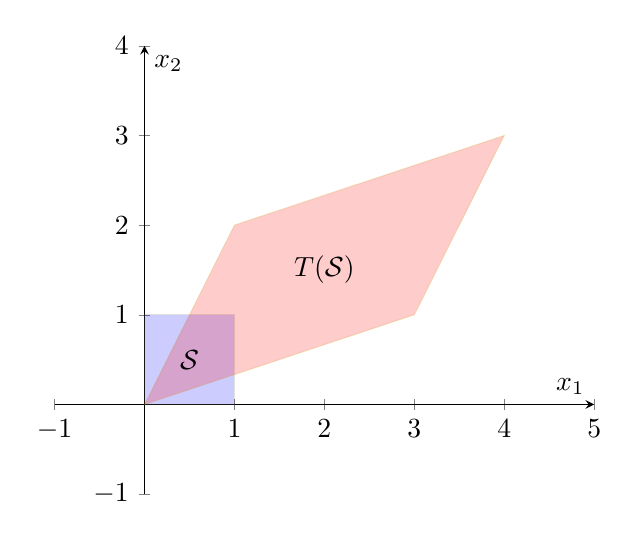
\begin{tikzpicture}
		\begin{axis}[xlabel=$x_1$, ylabel=$x_2$, axis x line=middle, axis y line=middle, xmin=-1, ymin=-1, xmax=5, ymax=4]

		\addplot[surf,mesh/rows=2, patch type=rectangle, blue, opacity=0.2] coordinates {(0,0) (1,0) (0,1) (1,1)};
		
		\addplot[surf,mesh/rows=2, patch type=rectangle, red, opacity=0.2] coordinates {(0,0) (1,2) (3,1) (4,3)};
		
		\node[draw=none, fill=none] at (axis cs:0.5,0.5) {$\mathcal{S}$} ;
		\node[draw=none, fill=none] at (axis cs:2,1.5) {$T(\mathcal{S})$} ;
		\end{axis}
	\end{tikzpicture}
	\caption{Grafische weergave van het voorbeeld}
	\label{fig:linafb}
\end{figure}